\documentclass[man]{apa2}
\usepackage{pslatex}
\usepackage{amssymb}
\usepackage{graphicx}
\usepackage{color}
\usepackage{covington}
\usepackage[usenames,dvipsnames]{xcolor}
\usepackage{booktabs}
\usepackage{setspace}
\usepackage{textgreek}
\usepackage{geometry}
\usepackage{pdflscape}
\usepackage{array}
\usepackage{floatrow}



\newcolumntype{C}[1]{>{\centering\let\newline\\\arraybackslash\hspace{0pt}}m{#1}}


\title{The trouble with quantifiers: Children's difficulty with ``some'' and ``none''}

\threeauthors{Alexandra C. Horowitz}{Rose M. Schneider}{Michael C. Frank}
\threeaffiliations{Department of Psychology, Stanford University}{Department of Psychology, Stanford University}{Department of Psychology, Stanford University}

\abstract{Using language requires speakers and listeners to make pragmatic inferences that extend beyond the literal sense of the utterance. For example, adult listeners quickly and easily infer from the utterance ``\textit{Some} of the cookies are oatmeal raisin'' that the others might not be. On the other hand, children have more difficulty with this statement; previous research has suggested that children succeed in making scalar implicatures using quantifiers in some cases but not others. Children's performance varies tremendously across studies and tasks however, limiting the number of possible direct comparisons between datasets. To address this issue, we designed a novel experimental paradigm, which both minimized task demands for participants, and enabled comparisons across different tasks. In Experiment 1, we used this paradigm to explore children's ability to compute both ad-hoc (contextual) and scalar (quantifier) implicatures, and found that while older 4-year-olds performed at ceiling for ad-hoc descriptions, they still performed poorly with scalar descriptions. Intriguingly, we also found bimodal and correlated performance with the quantifiers ``some'' and ``none''.  In Experiment 2, we attempted to isolate children's sources of difficulty with these terms by including only scalar trials, and found that while performance increased, it was still low. We also observed once again that children's success on ``some'' and ``none'' trials was positively correlated. In Experiment 3, we explored possible sources of developmental difficulty in this task, combining our paradigm with tests of inhibitory control and quantifier knowledge. After controlling for age, we found that inhibitory control did not predict the ability to make scalar implicatures, but that children who had difficulty with ``some'' and ``none'' in an implicature task also had issues with these terms in the quantifier knowledge task. Taken together, our results provide easily comparable developmental data on the development of pragmatic implicatures, and suggest that difficulty with scalar implicatures may in fact be rooted in a lack of quantifier knowledge. 
~\\

Keywords: pragmatics, development}

\shorttitle{The trouble with quantifiers}
\rightheader{The trouble with quantifiers}

\acknowledgements{We gratefully acknowledge Tamara Mekler for her assistance in data collection, the staff and families at Bing Nursery School, as well as David Barner for guidance on the Give-Quantifier task. 

~\\

\noindent Address all correspondence to Rose M. Schneider, Stanford University, Department of Psychology, Jordan Hall, 450 Serra Mall (Bldg. 420), Stanford, CA, 94305. Phone: 650-721-9270. E-mail: \texttt{rschneid@stanford.edu}.}

\begin{document}
\maketitle               

\section{Introduction}
%A cooperative speaker is one that produces utterances that are informative given their intended meaning. An implicature is an instance in which a weaker literal description (e.g., ``I ate some of the cookies'') implies that a stronger alternative (that I ate \emph{all} is not true, or else the cooperative speaker would have used the stronger description. \emph{Scalar} implicatures are ones that rely on lexical scales, or sets of related terms that are graded in meaning such as quantifiers (``some'' vs. ``all''), modals (``possibly'' vs. ``definitely''), logical connectives (``or'' vs. ``and'') and numerals (``one'' vs. ``two'') \cite{horn1972}. \emph{Ad-hoc} implicatures are contextually week descriptions that negate stronger interpretations (e.g., ``I ate the sugar cookies'' implies that I \emph{only} ate the sugar cookies, and not the other varieties available). \footnote{While \citeA{grice1975logic} distinguished ``generalized'' and ``particularized'' implicatures, this distinction has been controversial. Here we use ``ad-hoc implicature'' as a term of convenience to describe contextually-supported inferences while remaining agnostic about the theoretical distinction.}   While scalar and ad-hoc implicatures are similar in nature and simple for adults, they are often challenging for children. We investigate factors influencing children's pragmatic inferences across these types of descriptions.

In speech, adult listeners effortlessly make inferences that go beyond the literal sense of an utterance. For example, an adult who hears ``I ate \emph{some} of the cookies'' would expect that I did not eat \emph{all} the cookies, and left several for them. Similarly, an adult listener who hears ``I ate the sugar cookies,'' would most likely assume that I ate \emph{only} the sugar cookies, and not the other varieties. As implicatures, these two statements use a weaker literal description (in these cases, scalar and contextual, respectively) to imply that a stronger alternative is true. The first statement requires the listener to make a scalar implicature, which relies on lexical scales such as quantifiers (``some'' vs. ''all'') or modals (``possibly'' vs. ``definitely'') \cite{horn1972}. The second statement necessitates an ad-hoc implicature, in which a stronger description is negated by a contextually weaker description.\footnote{While \citeA{grice1975logic} distinguished ``generalized'' and ``particularized'' implicatures, this distinction has been controversial. Here we use ``ad-hoc implicature'' as a term of convenience to describe contextually-supported inferences while remaining agnostic about the theoretical distinction.} Previous research on children's on implicature comprehension has suggested that while children are able to make ad-hoc implicatures, they experience difficulty in computing scalar implicatures, and thus would have trouble inferring from ``I ate \emph{some} of the cookies'' that a few cookies still remain. Here, we explore the developmental trajectory of children's ability to make both ad-hoc and scalar implicatures, as well as investigate factors influencing children's performance across scalar descriptions. 

Children's processing of scalar implicatures, is an intriguing case study in pragmatic development. In contrast to adults' spontaneous and relatively automatic computation of scalar implicatures along quantifier lexical scales like  $<${\sc some, all}$>$, children's performance on these same scales is variable even until fairly late in development \cite{noveck2001}. However, it is possible that some of the paradigms used to test implicature comprehension in children might obscure their pragmatic abilities, such as ones that require children to make truth judgments for complex propositions. In fact, children show a graded pattern of successes and failures across different tasks \cite{guasti2005,papafragou2003, papafragou2004}. For example, five-year-olds asked to rate the felicity of a statement by selecting the magnitude of a reward (rather than making a binary true/false decision) assigned only mid-sized rewards for true but pragmatically odd descriptions \cite{katsos2011}, suggesting that they do recognize that weak statements are less felicitous than stronger ones.  Additionally, the wide range of methods and measures used to assess children's ability to compute implicatures does not allow for many direct comparisons in children's performance across different tasks (Table \ref{tab:lit_review}).

%This is pretty much directly copied
However, research on children's ability to compute scalar implicatures does indicate that their fragile performance may have less to do with their general pragmatic knowledge per se, and more to do with their knowledge of particular scales. The \emph{Alternatives Hypothesis}, proposed by Barner and colleagues \cite{barner2010, barner2011}, posits that children's ability to compute scalar implicatures relies on their recognition of the relevant lexical alternatives (e.g., that use of the weaker term ``some'' conveys a direct contrast with the stronger alternative ``all'', thus implying \emph{some but not all}).  In other words, children's pragmatic inferences rely on their ability to consider relevant possible alternative word choices that could have been used in place of the ones the speaker chose. So even in supportive paradigms, if children cannot bring to mind ``all'' when reasoning about ``some,'' they will fail to make an implicature.


\newgeometry{margin=1cm} 
\begin{landscape}
\begin{table}
\footnotesize
\centering
\begin{tabular}{| p{2.2cm} | p{2cm} | p{1.69cm} | p{4.5cm} | p{5cm} | p{7.2cm} |} \hline
{\bf Study} & {\bf Scale(s)} & {\bf Ages} & {\bf Measure} & {\bf Sentence Type} & {\bf Main Finding} \\ \hline
Noveck (2001) & non-necessity--necessity, possibility--impossibility, some--all & 5;1--5;11, 7;1--8;0, 9;0--9;5, 10;0--11;7 & Truth Value Judgment (\textit{Yes, I agree} or \textit{No, I do not agree}) & ``Some giraffes have long necks'' & \parbox[t]{7.2cm}{Comprehension matters: Children demonstrate\\ pragmatic competence by age 7 in evaluating a variety of plausible and implausible sentences.} \\ \hline
\parbox[t]{2.2cm}{Papafragou \&\\Mussolini (2003)} & \parbox[t]{2cm}{some--all,\\two--three,\\start--finish} & \parbox[t]{1.69cm}{4;11--5;11\\(Study 1)\\5;1--6;5\\(Study 2) } &  \parbox[t]{4.5cm}{Felicity Judgment (\textit{Did Minnie\\answer well?})} & ``Some of the horses jumped over the fence'' (when all of the horses jumped over the fence) & Support matters: Children were more likely to reject infelicitous weak descriptions for numbers, and for all types of weak descriptions in the task with more pragmatic support (informativeness training, context of competition, statements about specific events). \\ \hline
\parbox[t]{2.2cm}{Papafragou \&\\Tantalou (2004)} & some--all, ad-hoc, encyclopedic & 4;1--6;1 & Felicity Judgment (Decide whether or not to award a speaker a prize) & \textit{Did you color the stars?} ``I colored some (when all were colored) & Scales matter: Children mainly withheld prizes for weak descriptions, and at higher rates for ad-hoc trials than other trial types. \\ \hline
\parbox[t]{2.2cm}{Guasti, Chierchia, Crain, Foppolo, Gualmini,\\\& Meroni (2005)} & some--all & 7;0--7;7 & Truth Value Judgment: \textit{Yes, I agree} or \textit{No, I do not agree} (Studies 1--3), \textit{Did Carolina say the wrong thing?} (Study 4) & ``Some giraffes have long necks'' (replication of Noveck (2001)), and scene descriptions, e.g. ``Some monkeys are eating a biscuit'' (when all are) & Context matters: 7-year-olds reliably computer implicatures for ``some'' after a training that increased their sensitivity to the informativeness of speakers' descriptions (e.g., calling a grape ``fruit'' instead of ``grape'') and when contextualized as evaluating a novice speaker novice speaker describing a scene.\\ \hline
Miller, Schmitt, Chang, \& Munn (2005) & some--all & \parbox[t]{1.69cm}{4;1--5;5\\(Study 1)\\ 3;6--5;10\\(Study 2)} & \parbox[t]{4.5cm}{Direct Instruction Task\\(Study 1);\\Picture Matching Task\\(Study 2)} & ``Make some faces HAPPY/Make SOME faces happy/Make some HAPPY faces'' (Study 1), ``Shoe me where Pete made some faces HAPPY/Show me where Pete made SOME faces happy'' & Prosody matters: In both tasks (completing the scene or selecting the referent), children reliably identified only a subset of the faces (out of four) when ``some'' was stressed, but not when it was unstressed.\\ \hline
\parbox[t]{2.2cm}{Huang \&\\Snedeker (2009)} & \parbox[t]{2cm}{some--all,\\two--three} &\parbox[t]{1.69cm}{5;2--6;1\\(Study 1)\\5;5--6;9 \\(Studies 2\\\& 3)} & \parbox[t]{4.5cm}{Eye-tracking\\referent selection} & ``Point to the girl with some of the socks'' (when other girls and boys have shares of socks and soccer balls) & Time scale matters: Across studies, children were delayed in identifying the referent for scalar implicature trials, and accept and overlap between the meaning of ``some'' and ``all.'' \\ \hline
Katsos \& Bishop (2011) & some--all, ad-hoc & 5;1--6;3  & \parbox[t]{4.5cm}{Binary Truth Value Judgment\\(Study 1); Ternary Truth\\Value Judgment (Study 2);\\Sentence-to-picture Matching Task\\(Study 3)} & ``The mouse picked up some of the carrots'' & Measures matter: While children tended to a accept under-informative scalar and ad-hoc descriptions given a binary decision, they showed sensitivity to weaker statements given a ternary choice or picture matching task. \\ \hline
Barner, Brooks, \& Bale (2011) & some--all, ad-hoc & 4;0--5;0 &Truth Value Judgment & ``Are some of the animals sleeping?'' (when all are) & Specificity matters: 4-year-olds accept weak ad-hoc and scalar descriptions. When preceded by restrictive ``only'', they reject ad-hoc descriptions but continue to accept that ``only some'' can mean \emph{all}.\\ \hline
\parbox[t]{2.2cm}{Skordos \&\\Papafragou (2014)} & some--all & 4;9--5;8 & Felicity Judgment (\textit{Did the puppet answer well?}) & ``Some of the blickets have a crayon'' (when all of them do)  & Comparisons matter: Children were more likely to reject infelicitous uses of ``so'' if they first heard ``all'' falsely refer to quantity (only 3/4 blackouts had crayons), but not is ``all'' referred falsely to the objects (e.g., ``all of the blackest have a scarf'').\\ \hline \end{tabular} 
\caption{\label{tab:lit_review}Review of previous literature on children's comprehension of implicatures.} 
\end{table}
\end{landscape}
\restoregeometry

Previous research has supported this hypothesis, with children's performance in implicature tasks increasing when they have stronger access to lexical alternatives. Evaluating performance in competitions where alternative outcomes are salient \cite{papafragou2003} and using contextually-accessible (ad-hoc) scales (e.g., ``the cat and the cow are sleeping'' rather than ``some animals are sleeping''; \citeNP{barner2011}) both help preschoolers make implicatures. The Alternatives Hypothesis also predicts interactions between the supportiveness of a task and children's performance. For example, even three-year-olds show evidence of computing implicatures for ad-hoc contextualized scales when the task is a referential forced choice between possible interpretations \cite{stiller2014}.  Preschoolers also show some preliminary evidence of computing scalar implicatures for quantifiers in a similar forced-choice paradigm, albeit with prosodic support \cite{miller2005}. 

In sum, the Alternatives Hypothesis appears to provide a promising account of the current patterns of preschoolers' successes and failures in pragmatic implicature tasks. Nevertheless, work to date has varied widely in the particular scales, tasks, and measures used, as well as developmental samples that are relatively small while spanning several years of age. These concerns make it difficult to interpolate across findings and draw strong inferences about contrasts between contextually-supported (ad-hoc) and lexicalized (scalar) implicatures. In the current study, we create a paradigm which fills this gap, allowing exploration of children's processing of both ad-hoc and scalar implicatures with a single task.

In the current work, we designed a simple referent selection task in which children were asked to select which of three book covers they thought the experimenter was describing. Our design allowed us to fully counterbalance the trial types (ad-hoc vs. scalar descriptions crossed with implicature vs. unambiguous control targets) across participants, to examine both within-subject patterns of responses and between-subject developmental patterns, and to reduce the demands of the task by having children select the implied referent among three visual alternatives.

In Experiment 1, we included both ad-hoc and scalar descriptions with implicature and control trials for each. Four--year-olds were strong on ad-hoc trials \cite<similar to previous work, e.g.>{stiller2014}, but their performance on scalar implicature trials was very low. In Experiment 2, we ran the same task but replaced the ad-hoc trials with scalar trials. We found developmental increases in performance for each trial type, and higher performance on implicature trials for 4-year-olds in this scalar-only version of the task. Children's pattern of responses on scalar implicature trials was bimodal and strongly correlated with their performance on ``none'' (scalar control) trials, providing some clues about the factors underlying success in scalar implicatures. In Experiment 3, we explored two alternatives (inhibitory control problems and lack of quantifier knowledge) that could be contributing to children's difficulty with the quantifiers ``some'' and ``none''. Overall, our findings suggest that while preschoolers' computation of scalar implicatures can be supported by stronger recognition of the lexical alternatives, that their failure in making these implicatures may be rooted in an unclear and unestablished quantifier scale. 

\section{Experiment 1: Ad-hoc and scalar implicature computation in children}

Given the difficulty in equating results on children's computation of implicatures across different methods and paradigms, we created a single task that could be adapted to investigate both ad-hoc and scalar items in one task. This task involved one set of visual stimuli presented in the same order to all participants; however, the particular items (ad-hoc or scalar) queried were counterbalanced across participants. Thus, with one set of visual stimuli we could directly compare children's performance on both ad-hoc and scalar implicatures in a single experimental session. In Experiment 1, we included questions about ad-hoc and scalar implicatures within one session, and found that this paradigm was appropriate for ad-hoc items, but children still experienced difficulty computing scalar items.

% In Experiment 2, we included only scalar items in the task, and found that participants were moderately more successful at making implicatures when these trials were presented in isolation. In Experiment 3, we explored two alternatives potentially driving children's difficulties in this task.  

\subsection{Methods}

\subsubsection{Participants} A planned sample of 48 children was recruited from a university preschool. These children were drawn from two age groups: twenty-four 4.0 -- 4.5-year-olds (M = 4;2, median = 4.19, SD = 0.14) and twenty-four 4.5 -- 5.0-year-olds (M = 4.74, median = 4.73, SD = .16). Two children were excluded from the final sample for not completing the task, and one additional child was excluded due to experimenter error. All children's primary language was English, and no child completed more than one session of the task.  

\subsubsection{Stimuli}
Stimuli for all experiments were created to be appropriate for questions about both ad-hoc and scalar implicatures, allowing the experimenter to use one set of stimuli for both kinds of items in one experimental session. The experimental stimuli consisted of a set of printed pictures of three book covers with four familiar items on each cover. In each trial, one book cover contained four items of the same kind (e.g., four cats), another book cover contained four items of another kind (e.g., dogs), and the final cover contained two items of a new set and two items repeated from one of the other book covers (e.g., two birds and two cats). An example of the stimuli can be seen in Figure \ref{fig:demo}. All items on the book covers were familiar to children, and were able to be identified. All participants saw the same book covers in the same order. 


\begin{figure}
 \begin{center} 
  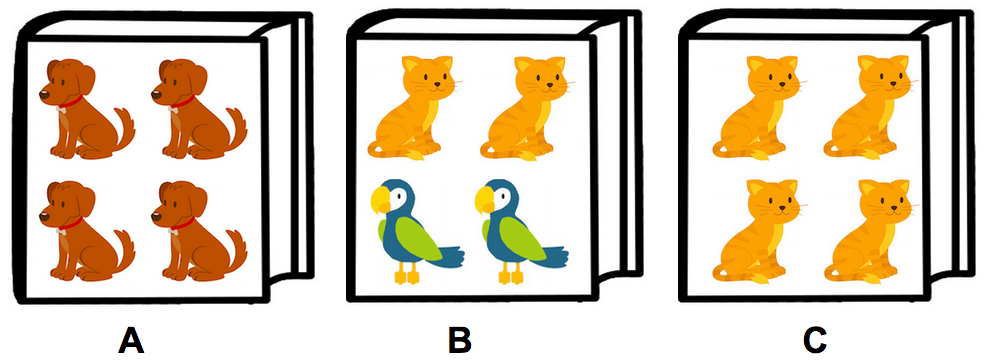
\includegraphics[height=2in]{figures/implicatures_demo_letters.png}
  \caption{\label{fig:demo} Example trial stimuli used in all experiments. Children received a clue from the experimenter about which book she had in mind and responded based solely on the clue; this was either an ad-hoc or a scalar description of a book with either an unambiguous or implicature target.} 
 \end{center} 
\end{figure}

\subsubsection{Procedure}
Participants were tested in individual sessions in a quiet room at their nursery school. The experimenter introduced the study as a guessing game, and explained that the child would receive a hint about which book cover the experimenter had in mind. In the instructions for the task, the experimenter emphasized that the child would only receive one clue about what book the experimenter was describing, and they had to use that clue to make their decision. All participants saw the book covers in the same order; however, three scripts with both ad-hoc and scalar trials were counterbalanced across participants. A breakdown of trial types and sample scripts can be seen in Table \ref{tab:scripts}. 

 \begin{table*}
 \footnotesize
 \centering 
     \begin{tabular}{C{1.5cm} C{2cm} C{1.5cm} C{1.5cm} C{4.5cm} C{1.5cm}} 
                      \hline 
       \null   Condition  & Trial type & \# trials, Expt. 1 & \# trials, Expts. 2 \& 3 & Statement: ``On the cover of my book, ...'' & Target   \\ 
       \hline  
            Scalar & implicature & 4 & 6 &  ``...some of the pictures are cats'' & B	 \\ 
          & all  & 2 &  6 & ``...all of the pictures are cats'' & C		                 \\
           & none  & 2 & 6 & ``...none of the pictures are cats'' & A			\\ 
               & unambiguous `some' 	&  2 &  & ``...some of the pictures are birds'' & B					        \\ 
	\hline
	    Adhoc       & implicature & 4 &  & ``...there are cats'' & C 		\\ 
	     & distractor & 2 &  & ``...there are dogs'' & A	     \\ 
          & comparison & 2 &  & ``...there are birds'' & B 	   \\
       \hline 
     \end{tabular} 
     \caption{Study designs for Experiments 1, 2, and 3, using script examples for the trial set pictured in Figure \ref{fig:demo}.  \label{tab:scripts} }
 \end{table*}
 

Prior to the test trials, children were familiarized to the task with a practice trial with three book covers, each displaying a single unique and familiar item.  During the practice trial, the experimenter told the child ``On the cover of my book, there's a TV,'' which corresponded to the middle book cover. After children had successfully completed the practice, they saw 18 test trials with stimuli of books containing sets of familiar items. At the start of every trial, the experiment would provide the child with either an ad-hoc or scalar description of one of the books and instruct the child to point to the book she was describing. If the child pointed to more than one book, or the response was otherwise ambiguous, the experimenter emphasized again that she was talking about just one book, and that they should choose the single book she was describing. 

In ad-hoc trials (eight total), the experimenter's descriptions of the target book used names of the pictured objects, providing contextual support for the target. Ad-hoc control trials referred to an unambiguous target (e.g., ``On the cover of my book, there are dogs'' in Figure \ref{fig:demo}), while implicature trials required the child to reason about the speaker's meaning given the ambiguous utterance (e.g., ``On the cover of my book, there are cats'', which could refer to either the book containing only cats or the book containing cats and birds). In these critical trials, children had to understand that the speaker could potentially be talking about either the book with four or two of the named object, but that by opting to describe only one kind of object she was referring to the cover with four of the same object; otherwise, she would have mentioned both kinds of objects, or the ones unique to that cover (i.e., birds). 

In scalar trials (ten total), the experimenter described the target book with quantifiers. For scalar items, control trials referred to unambiguous targets with the quantifiers ``all'' and ``none'' (e.g., ``On the cover of my book, \textit{all/none} of the pictures are cats'') or an unambiguous referent of ``some'' (e.g., ``On the cover of my book, \textit{some} of the pictures are birds''). On critical scalar implicature trials, the experimenter used the weak quantifier ``some'' to reference the item pictured across two book covers (e.g., ``On the cover of my book, \textit{some} of the pictures are cats''). These trials required the child to reason that because the speaker used the weak quantifier ``some'', she must be referring to the book picturing only two of the named target, or else she would have used the stronger quantifier ``all''. 

All participants saw image sets in the same order; however, these image sets were counterbalanced for target location across the three scripts. Description condition and trial-type were further randomized across participants, and were spaced to avoid immediate repeat trial types. Children did not receive feedback after the test trial.

\subsection{Results}


\begin{figure} 
 \begin{center} 
  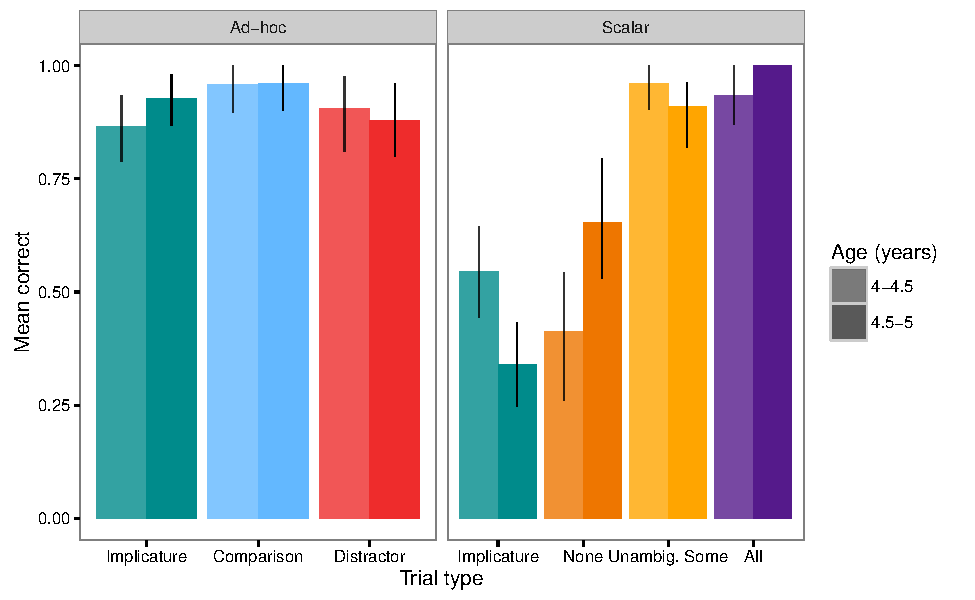
\includegraphics[height=2in]{figures/exp1_performance.pdf} 
  \caption{\label{fig:exp1_perf} Proportion of correct responses by each age group across all trial types and split by implicature type. Error bars show 95\% confidence intervals computed by non-parametric bootstrap. Children performed almost at ceiling in ad-hoc implicature conditions, but struggled in scalar trials, particularly in the ``some'' and ``none'' trials.} 
 \end{center} 
\end{figure}

Children's accuracy on all trial types is plotted in Figure \ref{fig:exp1_perf}. In implicature trials, children's performance was coded as correct if they selected the image consistent with either the ad-hoc or scalar inference. Children were at ceiling making ad-hoc implicatures, which is consistent with previous research suggesting that children are able to succeed in making such implicatures when they have access to the relevant lexical alternatives \cite{stiller2014}. Children's performance across ad-hoc trials provides strong evidence that our novel paradigm is an appropriate measure for such items.

In contrast to their success in making ad-hoc implicatures, children struggled in scalar trials. Although they succeeded in ``all'' and ``unambiguous some'' trials, children performed at chance on ``some'' trials (4--4.5-year-olds: \emph{t}(22) = .4, \emph{p} = .72; 4.5--5-year-olds: \emph{t}(24) = -2, \emph{p} =  .06) and at chance on ``none'' trials (4--4.5-year-olds: \emph{t}(24) = -.9, \emph{p} = .4; 4.5--5-year-olds: \emph{t}(24) = 1.6, \emph{p} = .13). 
	
%This is lifted directly from Ali's cogsci paper
In a planned analysis, we ran a logistic mixed effects model, predicting a correct response as an interaction of age, condition (ad-hoc or scalar) and trial type (implicature or control), with random effects of participant and trial type. We found that performance was slightly lower for scalar trials than ad-hoc trials ($\beta$= --8.02, \textit{p} = .09), and that there was a significant interaction between condition and trial type, such that performance was significantly worse on scalar implicature trials ($\beta$= 16.45, \textit{p} \textless  .02). We also found a significant 3-way interaction between condition, trial type, and age, such that performance on scalar implicature trials decreased with age ($\beta$ = --4.16, \textit{p} \textless  .01). There were no significant effects of adding trial order (trials in the first half vs. second half of the experiment), indicating that performance did not change throughout the course of the experiment. 

 \begin{figure}[!h]
 	\centering
           \begin{floatrow}
             \ffigbox{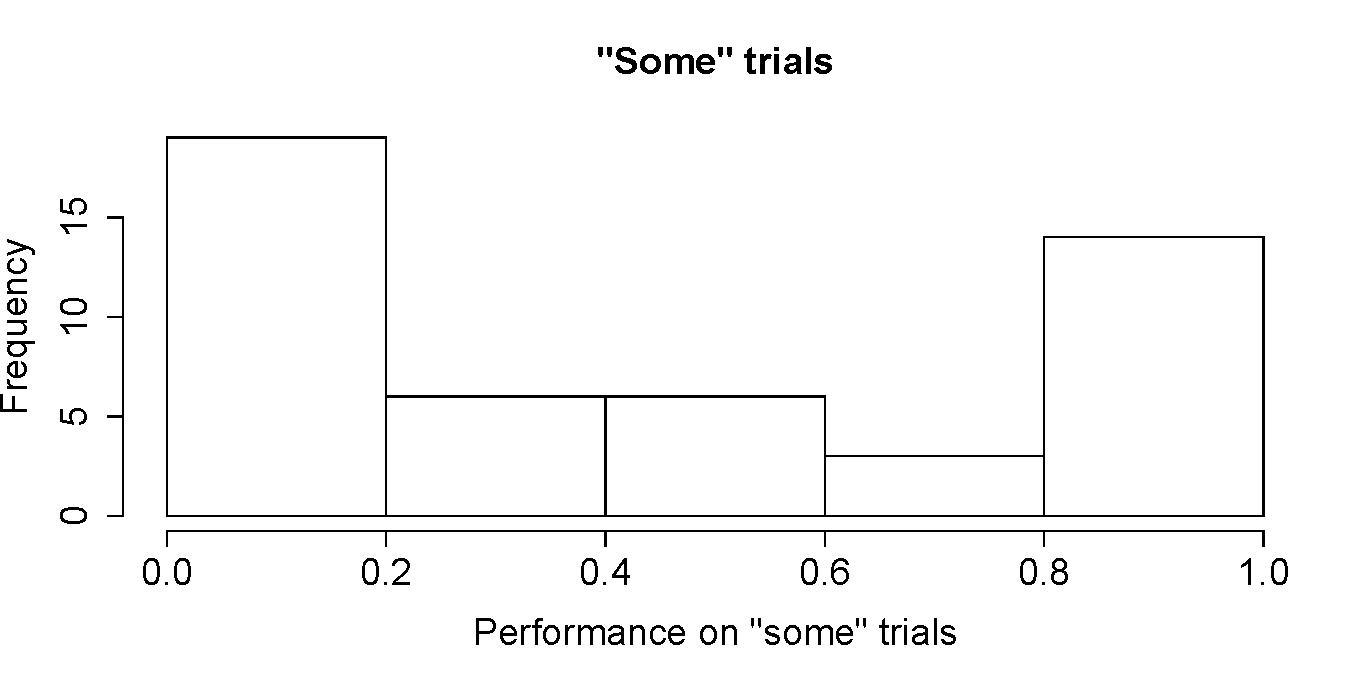
\includegraphics[scale = 0.33]{figures/exp1_imphist.pdf}}{\caption{Histogram of performance on ``some'' trials}\label{fig:imp_hist}}
             \ffigbox{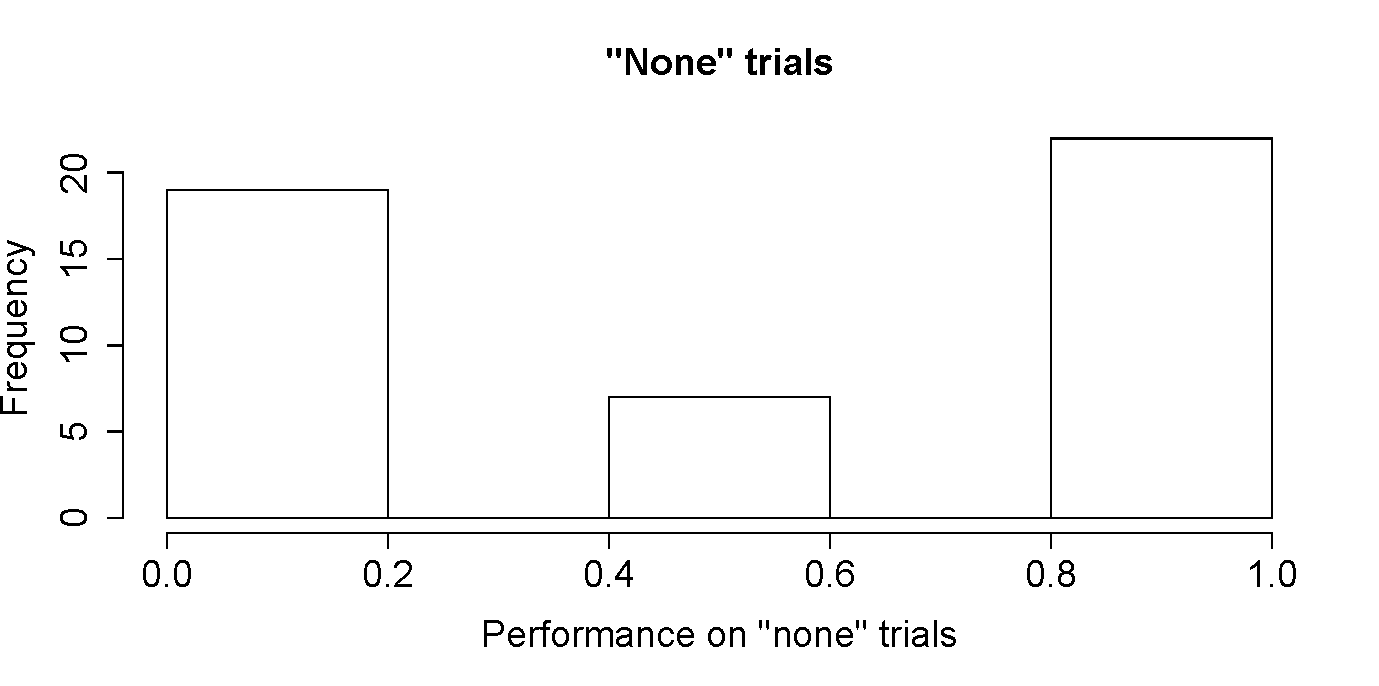
\includegraphics[scale = 0.33]{figures/exp1_nonehist.pdf}}{\caption{Histogram of performance on ``none'' trials}\label{fig:none_hist}}
           \end{floatrow}
\end{figure}	


\begin{figure} 
 \begin{center} 
  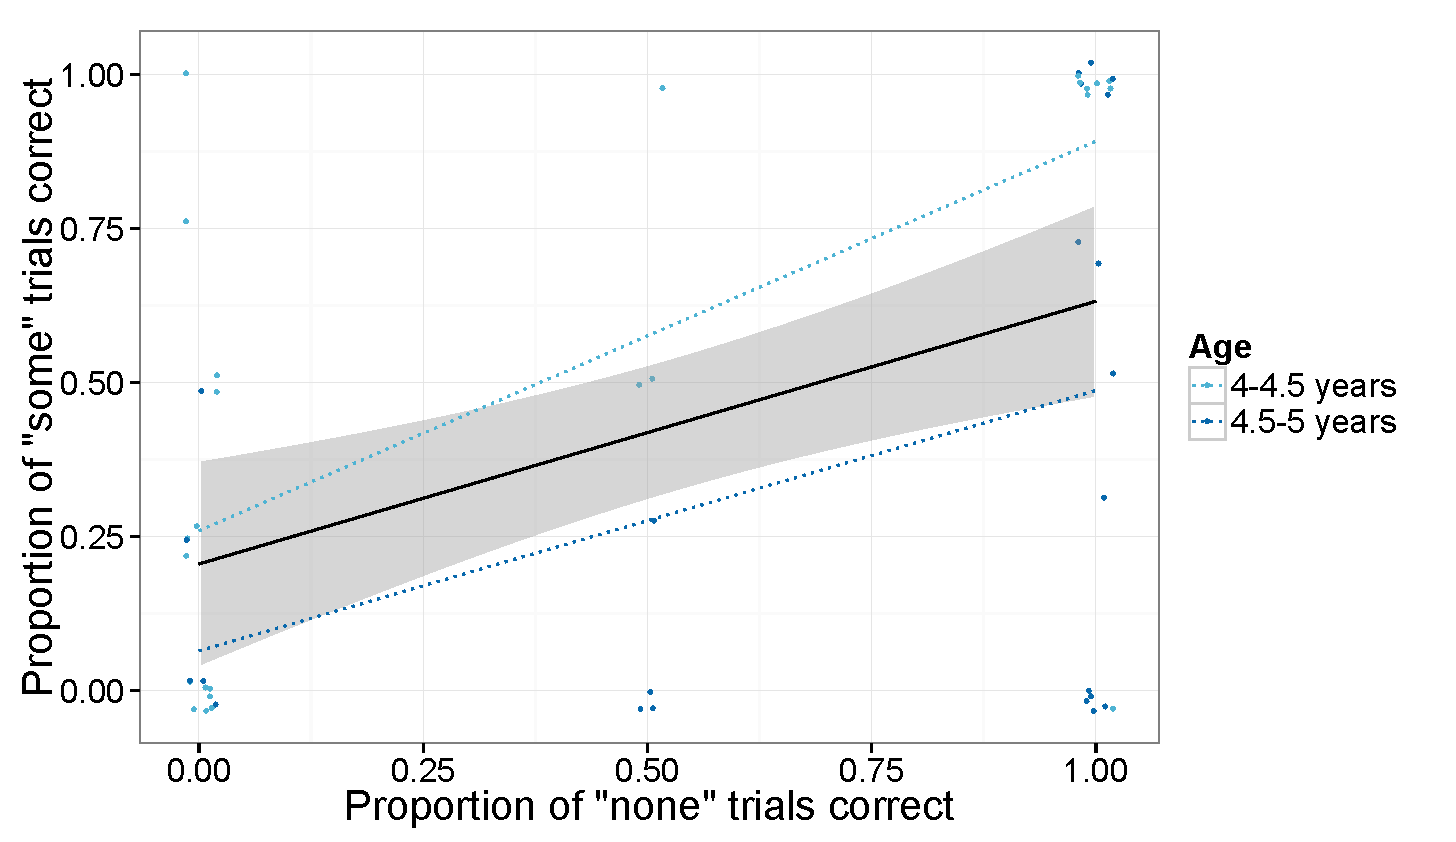
\includegraphics[height=2.5in]{figures/exp1_diffs.pdf} 
  \caption{\label{fig:exp1_diffs} Scatterplot relating individuals' performance on ``some'' and ``none'' trials per age group in Experiment 1. The aggregate trend is plotted in black along with its 95\% confidence interval, and trends for individual age groups are shown by dotted lines. Points are jittered slightly to avoid over plotting} 
 \end{center} 
\end{figure}

In post-hoc analysis of the data, we found an unpredicted consistency in performance on ``some'' and ``none'' (Figures \ref{fig:imp_hist} and \ref{fig:none_hist}).\footnote{We also observed this bimodal performance in pilot testing, and found that it replicated in Experiment 1}  To examine their patterns of responses more closely, we ran Hartigan's dip test and found significant bimodal distributions for both \textit{some} (\textit{D} = .15, \textit{p} \textless  .0001) and \textit{none} (\textit{D} = .20, \textit{p} \textless  .0001). This suggests children did not respond at chance in scalar trials, but consistently either correctly or incorrectly. Additionally, children's success on \textit{some} and \textit{none} trials was highly correlated (\textit{r} = .47, \textit{p} \textless  .001), such that children who performed better on some trials also tended to perform better on none trials (Figure \ref{fig:exp1_diffs}).  Performance on \textit{none} and \textit{all} trials (\textit{r} = .11, \textit{p} = .45) and \textit{some} and \textit{all} trials (\textit{r} = .01, \textit{p} = .95) was not correlated. 

\subsection{Discussion}

The results of Experiment 1 indicated that while children were easily able to make ad-hoc implicatures in our task, they had difficulty making scalar implicatures. This pattern of performance was puzzling, given both our efforts to reduce task demands and children's striking success in ad-hoc trials. Despite having access to both visual alternatives (the three selection choices) within each trial and lexical alternatives across all trials, children were still at chance in making scalar implicatures in our task. 

Even more intriguing was the unexpected developmental change we observed on \textit{none} trials. We included ``none'' as an unambiguous control quantifier, but found that children performed at chance for this scalar term as well. These results are supported by previous work suggesting that even older preschoolers struggle with negation occurring in arbitrary contexts \cite{nordmeyer2014}. Given children's difficulty with ``none'' and the strong positive correlation between \textit{some} and \textit{none} trials, it is possible that making implicatures necessitates some familiarity with both ends of the quantifier scale (\textit{none -- some -- all}). In addition to understanding the extremes of the quantifier scale, two other possibilities -- namely, lack of quantifier knowledge, and inhibitory control -- may also account for children's decreased performance on scalar items. However, we wondered if these results were the effect of including both ad-hoc and scalar quantifier descriptions within one experimental session. It is possible that children's success on ad-hoc trials may have to a misinterpretation of a scalar description (e.g., ``On the cover of my book, some of the pictures are cats'') to an ad-hoc one (``On the cover of my book, there are cats''). 

To further explore the possibility that children's performance on scalar trials might have been influenced by ad-hoc trials, we removed all ad-hoc trials from our task, and ran a scalar-only version of the the study.

\section{Experiment 2: Isolating scalar implicatures}
In Experiment 2, we pursued the possibility that children might be failing in making scalar implicatures as a result of competing ad-hoc descriptors contained in the same experimental session. Additionally, we expanded our sample age-range to 3--5 years in order to more fully explore the developmental trajectory of scalar implicature comprehension. 

\subsection{Methods}
\subsubsection{Participants} 

We recruited a new sample of 50 participants from a university preschool: twelve 3.0--3.5-year-olds (M=3;4, median = 3.35, SD = 0.1), twelve 3.5--4.0-year-olds (M=3;8, median = 3.67, SD = .12), fourteen 4.0--4.5-year-olds (M=4;3, median = 4.24, SD = .1), and twelve 4.5--5.0-year-olds (M=4;8, median = 4.63, SD = .15). One additional child was excluded for stopping the task early.

\subsubsection{Stimuli}
Stimuli were identical to Experiment 1. The only changes made in experimental protocol were to the scripts;  all 18 test trials were converted to quantifier descriptions (Table \ref{tab:scripts}). In Experiment 2, the 18 test trials consisted of six control \textit{all} trials (e.g., ``On the cover of my book, \textit{all} of the pictures are cats''), six \textit{none} trials (e.g., ``...\textit{none} of the pictures are cats''), and six scalar implicature trials (``...\textit{some} of the pictures are cats''). We removed the unambiguous \textit{some} trials to more effectively counterbalance; in ``some'' trials, the quantifier always referenced the item pictured across two book covers (e.g., in Figure \ref{fig:demo}, children heard references to \textit{none, some,} or \textit{all} cats). As in Experiment 1, image sets were presented in a fixed order, counterbalanced for both target location and triad order. Participants were randomly assigned to one of three scripts, with a pseudo-randomized trial order such that every book set was referred to by each quantifier type, and the same trial type never immediately repeated.

\subsubsection{Procedure}
The procedure was identical to Experiment 1. 

\subsection{Results}

\begin{figure} 
 \begin{center} 
  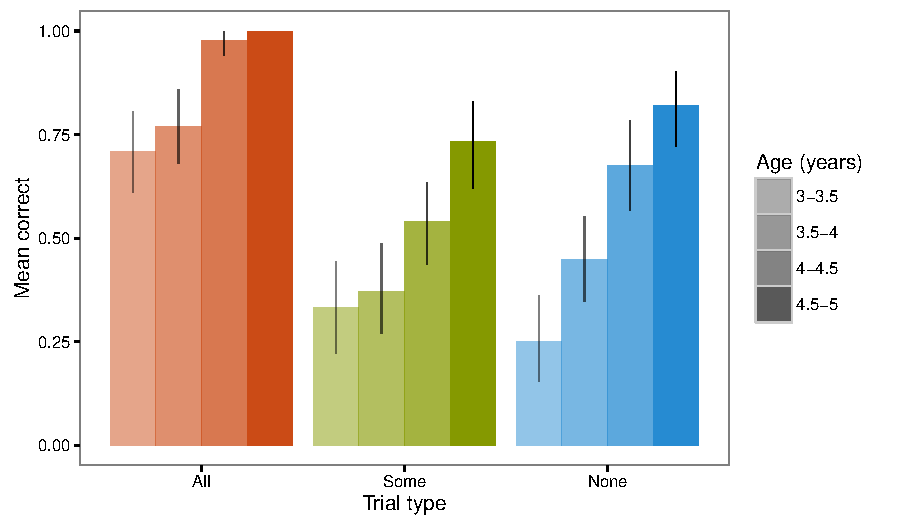
\includegraphics[height=2in]{figures/exp2_performance.pdf} 
  \caption{\label{fig:exp2_perf} Proportion of correct responses by each age group across all scalar trial types.  Error bars show 95\% confidence intervals computed by non-parametric bootstrap.} 
 \end{center} 
\end{figure}

In Experiment 2, children's performance increased with age (Figure \ref{fig:exp2_perf}). Performance was highest in \textit{all} trials, with all age groups significantly above chance (\emph{p} $<$ .05 for all tests). However, performance was still low in both \textit{none} and \textit{some} trials, with only 4.5--5-year-olds group performing above chance for \textit{none} trials (\textit{t}(11) = 3.09, \textit{p} $<$ .01) and only marginally above chance in \textit{some} trials (\textit{t}(11) = 1.85, \textit{p} $<$ .09). Children's performance in Experiment 2 was not significantly different than in Experiment 1, in independent sample t-tests by trial type between age groups in both experiments (\emph{p} $>$ .09 for all tests). 

We ran a planned logistic mixed effects model, predicting correct responses as an interaction of age and trial type (\textit{all, some}, or \textit{none}), with random effects of trial type by participant. However, we found that the only significant effect that emerged was age, such that performance increased across trials as children got older ($\beta$ = 20, \textit{p} \textless  .001). Adding trial order (first or second half of the experiment) to the model did not interact with any of the variables, indicating the performance did not change over the course of the experiment. 

Consistent with the findings from Experiment 1 model, we  ran Hartigan's dip test and again found significant bimodal patterns of responses for both \textit{some} (\textit{D} = .12, \textit{p} \textless  .0001) and \textit{none} (\textit{D} = .15, \textit{p} \textless  .0001) trials. Once again, these trial types were highly correlated with one another (\textit{r} = .52, \textit{p} \textless  .001). 

As an exploratory analysis, we ran another version of the mixed effects model removing the random effect of trial type, as this model does not find trial type effects due to correlation observed between trial types. In addition to a main effect of age (\textit{t} = 1.88, \textit{p} \textless  .01), this model revealed that performance on \textit{some} trials was lower than \textit{all} trials (\textit{t} = --7.69, \textit{p} \textless  .01), and marginally reduced from \textit{none} trials (\textit{t} = 3.03, \textit{p} = .09). We also found interactions between trial type and age however, such that there was a greater difference between younger children's performance on \textit{some} and \textit{all} trials (\textit{t} = 2.84, \textit{p} \textless  .001), and \textit{some} and \textit{none} trials (\textit{t} = 0.90, \textit{p} = .05). Overall, these findings indicate that while young children struggle with the quantifiers ``some'' and ``none,'' comprehension of these terms is more variable earlier in development in relation to ``all.'' 

\begin{figure} 
 \begin{center} 
  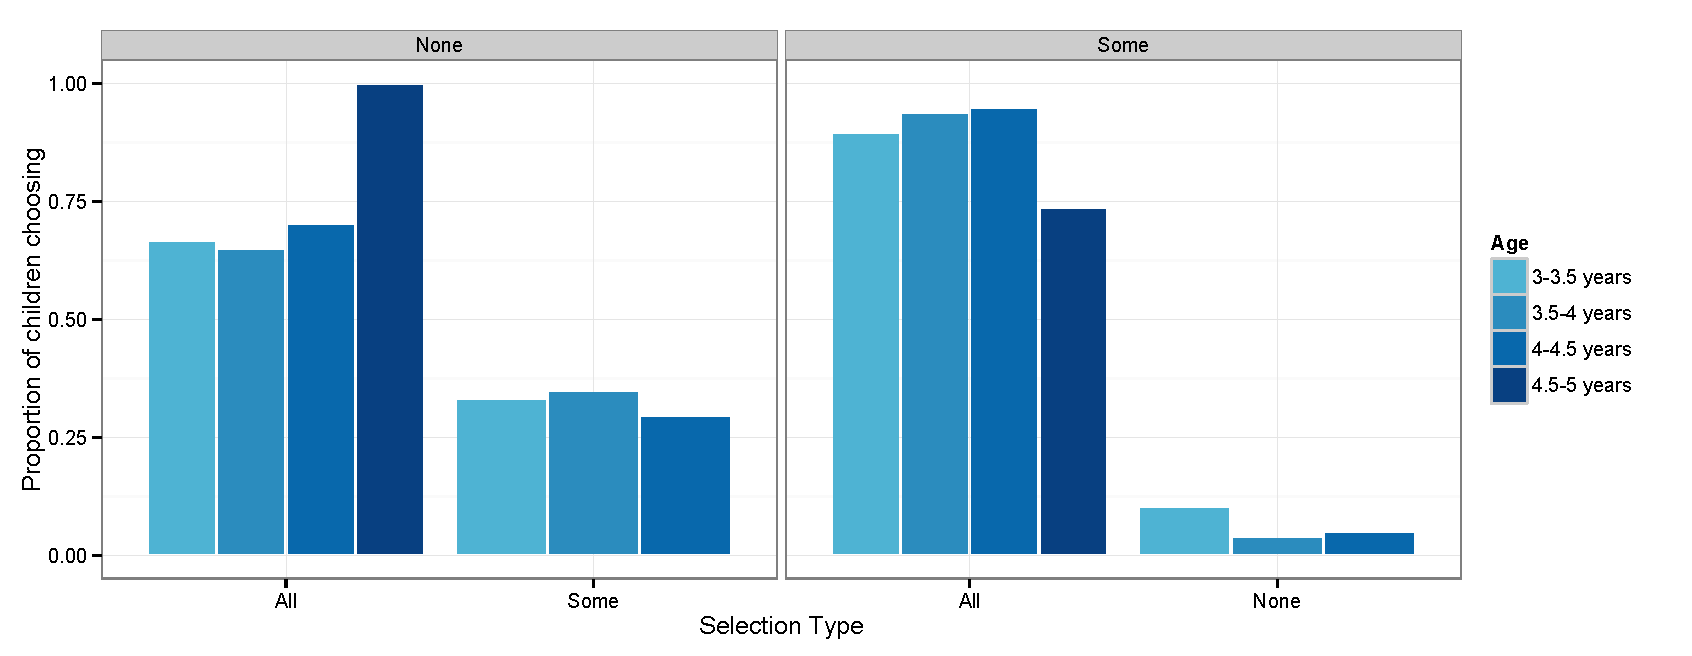
\includegraphics[height=2in]{figures/exp2_wrong.pdf} 
  \caption{\label{fig:exp2_wrong} Proportion of children choosing an alternative on incorrect ``some'' and ``none'' trials.} 
 \end{center} 
\end{figure}

In a further exploratory analysis, we were interested in the particular kinds of errors that children made in ``some'' and ``none'' trials (Figure \ref{fig:exp2_wrong}). We found that on these trials children matched the noun on both kinds of trials, and chose the ``all'' option more frequently, indicated some evidence for either listening through the quantifier (i.e., an issue of inhibitory control), or misunderstanding what the quantifier meant (a lack of quantifier knowledge). 


\subsection{Discussion}

In Experiment 1, we observed success in children's computation of ad-hoc, but not scalar implicatures. To explore whether children's performance in making scalar implicatures was hindered by the presence of both ad-hoc and scalar items in the same session, we excluded ad-hoc items, and replaced them with scalar descriptions. 

When faced with only scalar implicatures, children's performance was marginally (although not significantly) better than in Experiment 1, with success in making a scalar implicature positively correlated with age. We still observed low performance in both the \textit{some}, as well as the unambiguous \textit{none} trials. Additionally, we again found bimodal and correlated patterns of responses in these two trials, with children making errors in i``some'' trials also failing on ``none'' trials. 

The results of Experiment 2 indicated that children have difficulty with making scalar implicatures beyond dealing with competing contextual descriptors, but the cause of this developmental change is not clear. One possible explanation for this effect is that children's knowledge of the full quantifier scale is not yet adult-like in their preschool years, and that the meanings of these scalar terms may yet be established. Another possibility is that children's performance might suffer on these task from developing inhibitory control, with children not being able to overcome the impulse to select the target noun, regardless of the quantifier used. We explore these two alternatives in Experiment 3, and include measures of both inhibitory control and quantifier knowledge in the same session. 

%Need to make a better individual differences graph for this, also need to make a graph for what kinds of errors kids make
				
\section{Experiment 3: Inhibitory control and quantifier knowledge measures}

In an effort to explore the particular sources of difficulty for children in making scalar implicatures, in Experiment 3 we supplemented our implicature task with an inhibitory control task, the Dimensional Change Card Sort (DCCS) \cite{zelazo2006}, and a quantifier-knowledge task, Give-Quantifier \cite{barner2009} in a within-subjects design.  

\subsection{Methods}
\subsubsection{Participants} We recruited a new planned sample of 72 children from a university preschool; this sample was selected to have 80\% power to detect correlations of \emph{r} = .32. Once again, we included children from 3--5 years: twenty-one 3--3.5-year-olds (M = 3.27, median = 3.28, SD = 0.15), fifteen 3.5--4-year-olds (M = 3.79, median = 3.82, SD = 0.15), nineteen 4--4.5-year-olds (M= 4.17, median = 4.11, SD = 0.13), and seventeen 4.5--5-year-olds (M = 4.71, median = 4.68, SD = 0.14). Twelve children additional were recruited but excluded from the final sample for having participated in either Experiments 1 or 2. Nine children completed one of the three tasks in a subsequent testing session. 

\subsubsection{Stimuli} The stimuli for the implicature task were identical to Experiment 2. Our measure of inhibitory control was the Dimensional Change Card Sort (DCCS, \cite{zelazo2006}), with materials drawn from that study. The 14 laminated sorting cards used in the study consisted of 7 red rabbits and 7 blue boats. These cards were put into plastic sorting trays, one with a red boat, and the other with a blue rabbit. To assess quantifier knowledge, we used the Give-Quantifier task \cite{barner2009}. Stimuli for this task consisted of three different sets of plastic fruits (8 oranges, 8 bananas, and 8 strawberries) and a red plastic plate. These fruits were grouped together by kind at the start of each trial. 

\subsubsection{Procedure}
The procedure for our implicature task was identical to Experiment 2. Task order was counterbalanced across participants, and individual scripts for each task were also counterbalanced to avoid any possibility of order effects. The tasks were done in a small room apart from the main classroom in individual sessions. The experimenter asked the child before the start of every task whether she would like to play the game or return to the classroom. 

We drew our protocol for DCCS directly from the original methods paper \cite{zelazo2006}. Our only modifications to the the task to eliminate the extended version of the game, and to score children based solely on their answer without recording reaction time.  

In running the Give-Quantifier task, we followed the methods of the original paper \cite{barner2009}, with the exception of the quantifiers used in the task (\textit{some, all, none} and \textit{most}). The experimenter used the partitive construction and prosodically emphasized the quantifier equally across all trials (e.g., ``Can you put \textit{all} of the bananas into the circle?''). Quantifiers were presented in two different orders between participants, and fruit-quantifier pairings were quasi-randomized such that the same pairing was not repeated within a session. If the child request clarification, the experimenter repeated the prompt, and added that the child should put however many pieces of fruit she felt should go on the plate. 

In coding the results of the Give-Quantifier task, we relied on the original coding scheme \cite{barner2009}; \textit{all} and \textit{none} trials were coded as correct for 8 and 0 pieces of fruit given respectively, whereas \textit{some} trials were coded as correct if the child gave between 2 and 7 pieces, and \textit{most} trials were correct if the child gave between 5 and 7 pieces. 

\subsection{Results}

\begin{figure} 
 \begin{center} 
  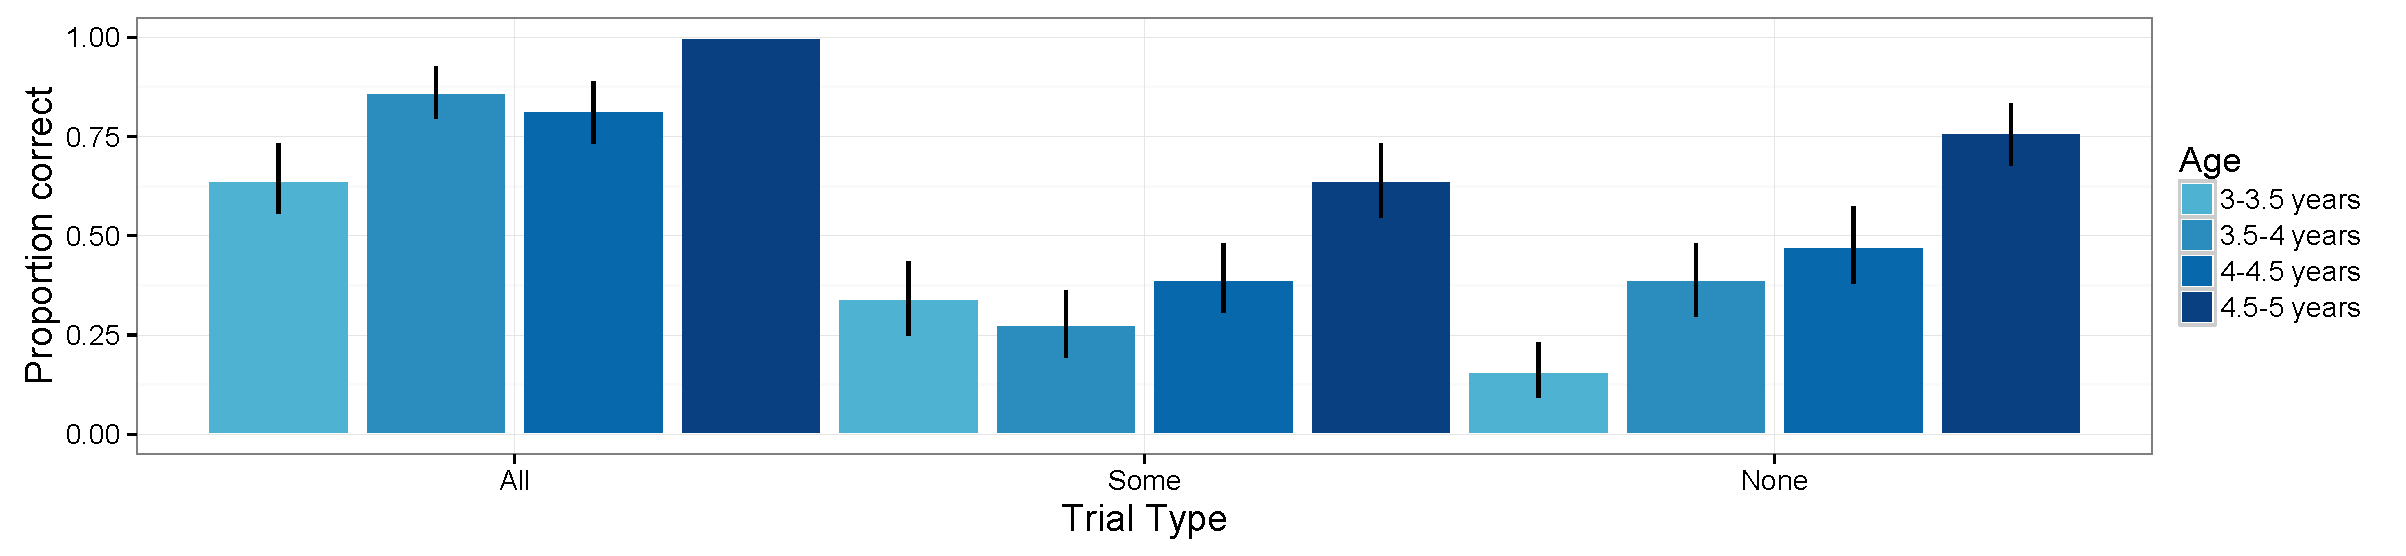
\includegraphics[height=2in]{figures/exp3_performance.pdf} 
  \caption{\label{fig:exp3_perf} Proportion of correct responses by each age group across all scalar trial types.  Error bars show 95\% confidence intervals computed by non-parametric bootstrap.} 
 \end{center} 
\end{figure}

We again replicated children's performance on our implicature task (Figure \ref{fig:exp3_perf}); independent sample t-tests between performance in Experiments 2 and 3 within age-groups did not yield any significant differences (\emph{p} $>$ .1 for all tests) except for 4--4.5-year-olds' performance on ``all'' trials, which was significantly lower in Experiment 3 (\emph{t}(31), \emph{p} $<$ .05). Once again, we found that performance increased with age, with the 4.5--5-year-olds the only group performing significantly above chance on \emph{none} trials, (\emph{t}(16) = 3.75, \emph{p} $<$ .002), but still performing near chance on \textit{some} trials (\emph{t}(16) = 1.18 \emph{p} = .26). As in Experiment 2, we ran Hartigan's dip test in a post-hoc analysis and again found a significant bimodal distribution of performance in both \textit{some} (\textit{D} = .07, \textit{p} = .002) and \textit{none} trials (\textit{D} = .15, \textit{p} $>$ .0001). Performance with these two quantifiers was also significantly positively correlated (\emph{r} = .4, \emph{p} $<$ .001). However, because children's performance was so highly correlated with age, we ran a partial correlation controlling for age, and found both these trials were still significantly correlated (\emph{r} = .3, \emph{p} $<$ .01). 

%logistic model

\begin{figure} 
 \begin{center} 
  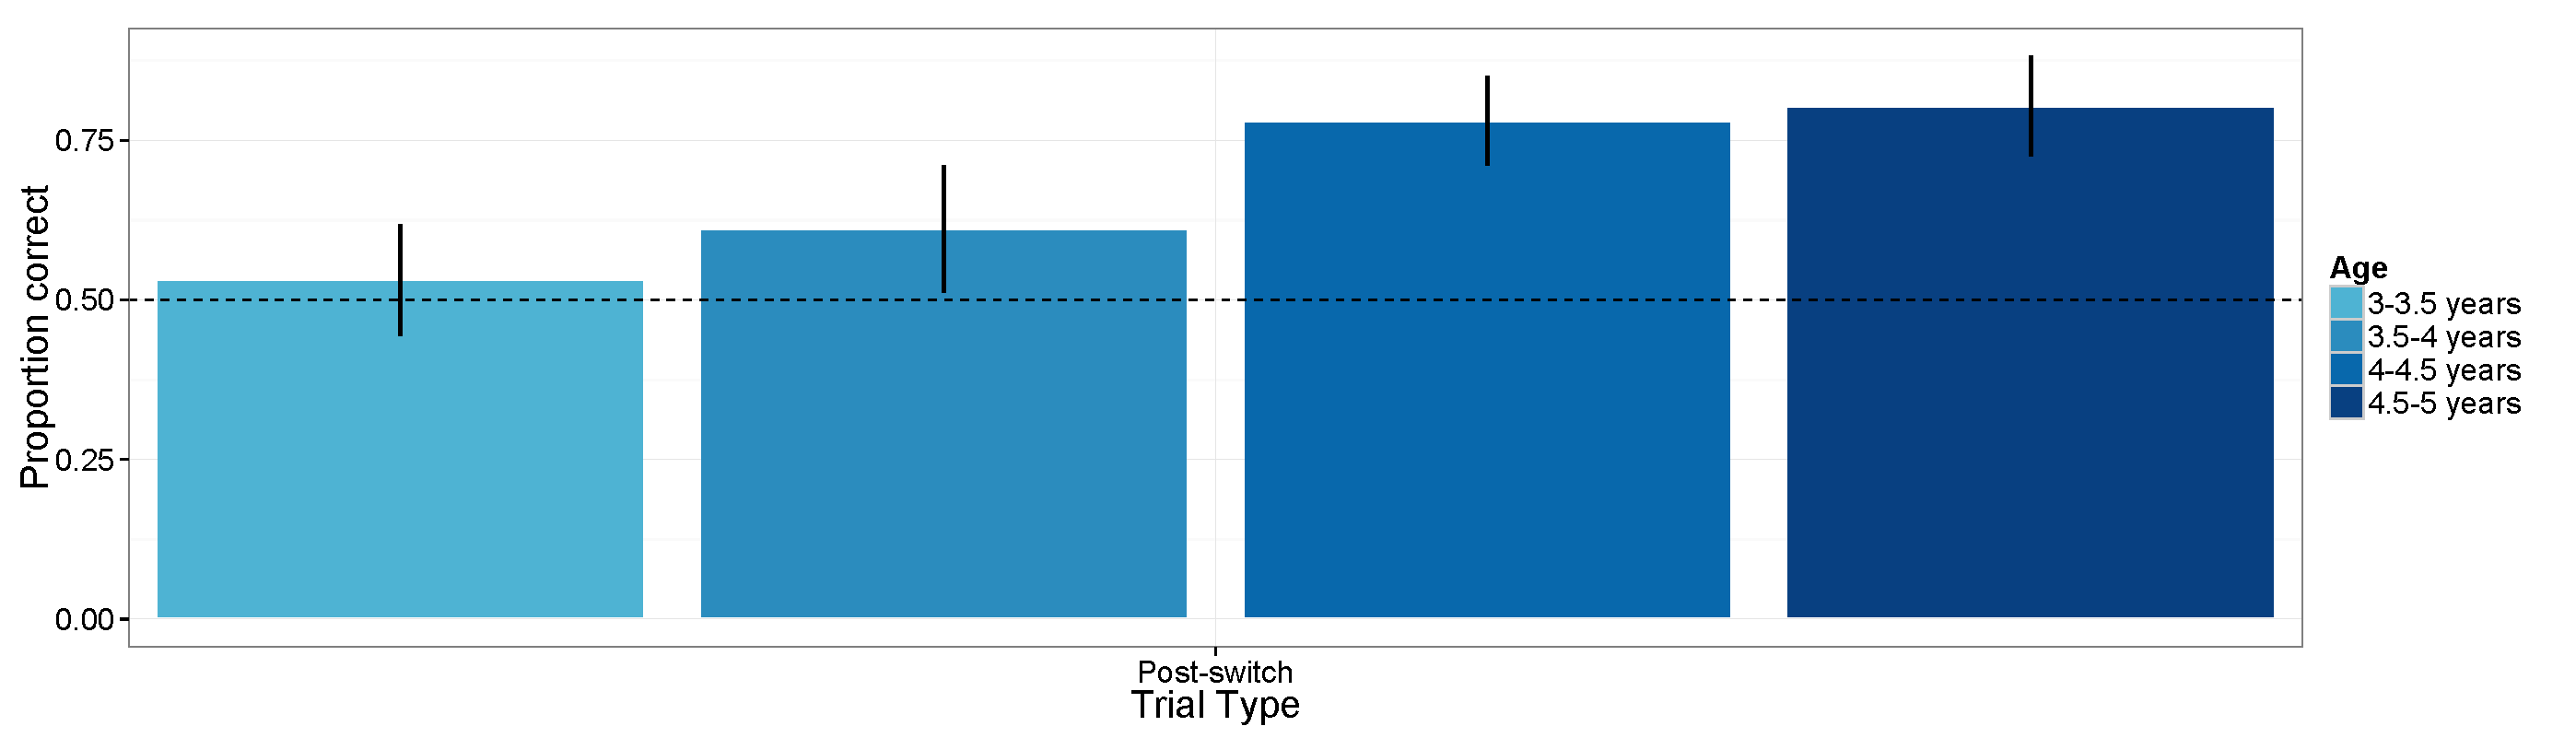
\includegraphics[height=2in]{figures/DCCS.pdf} 
  \caption{\label{fig:exp3_DCCS} Proportion of correct responses by each age group in both pre- and post-switch trials.  Error bars show 95\% confidence intervals computed by non-parametric bootstrap.} 
 \end{center} 
\end{figure}

We next turned to whether children's lower and correlated performance on \emph{some} and \textit{none} trials was a result of difficulty with inhibitory control. Accuracy on the DCCS is plotted in Figure \ref{fig:exp3_DCCS}. This task was significantly correlated with age (\textit{r} = .28, \textit{p} = .018), with only 4--5-year-olds performing significantly better than chance (4--4.5-year-olds: \emph{t}(18) = 3.05, \emph{p} $<$ .01; 4.5--5-year-olds: \emph{t}(16) = 3.31, \emph{p} $< $.01). After controlling for age, we did not find any significant correlation between inhibitory control and performance on either \textit{some} trials (\textit{r} = .13, \textit{p} = .26) or \textit{none} trials (\textit{r} = - .01, \textit{p} = .93) in our implicature task.

\begin{figure} 
 \begin{center} 
  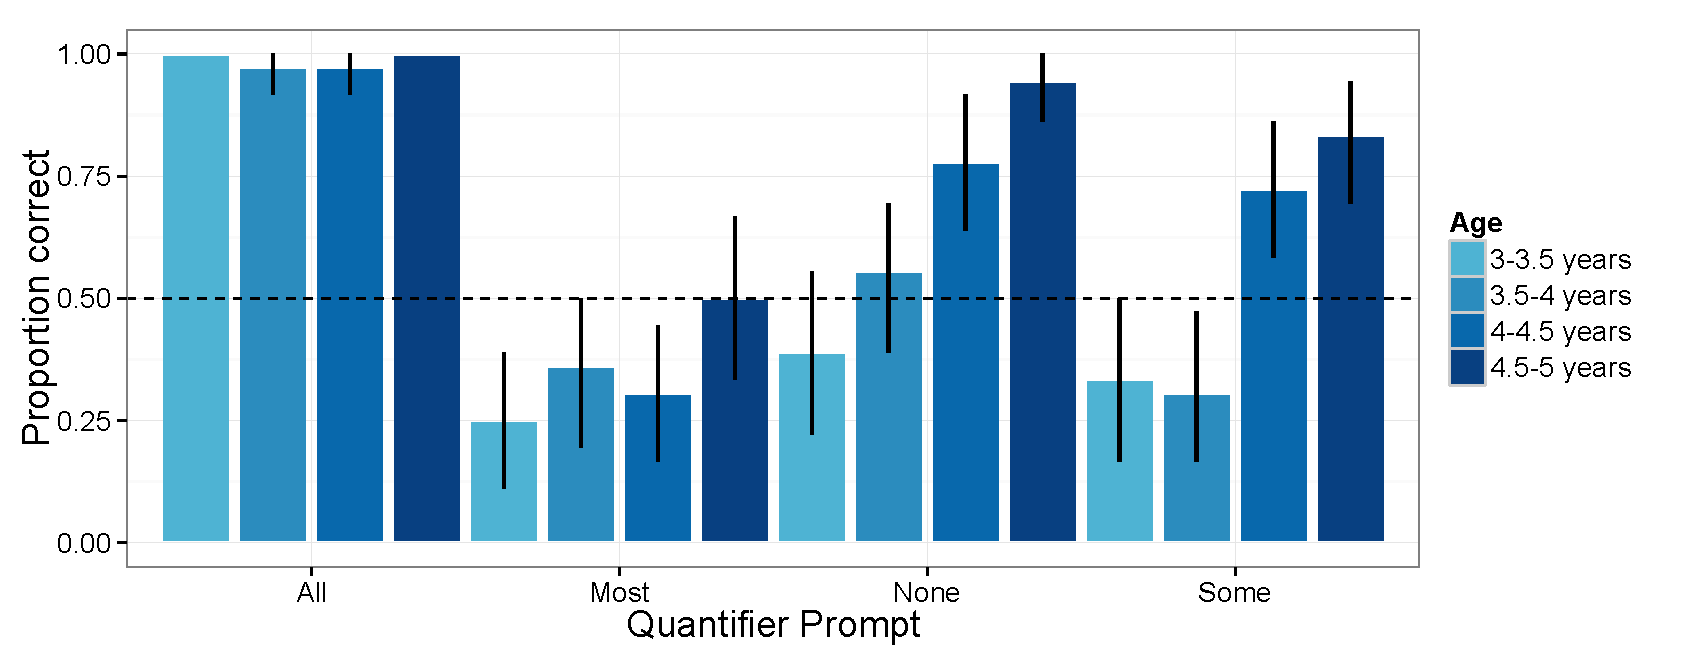
\includegraphics[height=2in]{figures/exp3_GQright.pdf} 
  \caption{\label{fig:exp3_GQright} Proportion of correct responses by each age group for quantifier prompts \textit{all, most, none} and \textit{some}.  Error bars show 95\% confidence intervals computed by non-parametric bootstrap.} 
 \end{center} 
\end{figure}

Another hypothesis for the pattern of results we observed in our implicature task was that children tested had not yet established a consistent quantifier scale; we therefore included the Give-Quantifier task in our experimental sessions. Children's performance on this task was very similar to performance on our implicature task, with all age groups performing at ceiling for the prompt \textit{all}, and only older children succeeding on with the prompts \textit{most, none} and \textit{some}. Figure \ref{fig:GQ_spread} shows the breakdown of how children responded to these scalar terms. We collapsed across all age groups and found a significant bimodal distribution of responses with Hartigan's dip test in both ``some'' (\emph{D} = .19, \emph{p} $<$ .0001) and ``none'' trials (\emph{D} = .15, \emph{p} $<$ .0001).  In an exploratory analysis, we ran dip tests by age group, and found that this effect was primarily driven in ``some'' trials by 3--3.5-year-olds (\emph{D} = .14, \emph{p} $<$ .0004) and 4--4.5-year-olds (\emph{D} = .13, \emph{p} $<$ .004), and in ``none'' trials by 3--3.5-year-olds (\emph{D} = .21, \emph{p} < .0001) and 3.5--4-year-olds (\emph{D} = .2, \emph{p} $<$ .0001).  Overall, we found that younger children showed a bimodal pattern of response to the prompt \textit{none}, with the majority of children giving 0 or 8 items in these trials, gradually shifting to a correct response by 4.5--5 years. Similar to performance with \textit{some} trials in our implicature task, we found a large proportion of younger children giving all 8 objects in response to the prompt \textit{some}, and the oldest age groups giving a more adult-like response. In a partial correlation controlling for age, we found that performance in \emph{none} and \emph{some} trials was significantly correlated (\textit{r} = .61, \textit{p} \textless .0001). 

\begin{figure} 
 \begin{center} 
  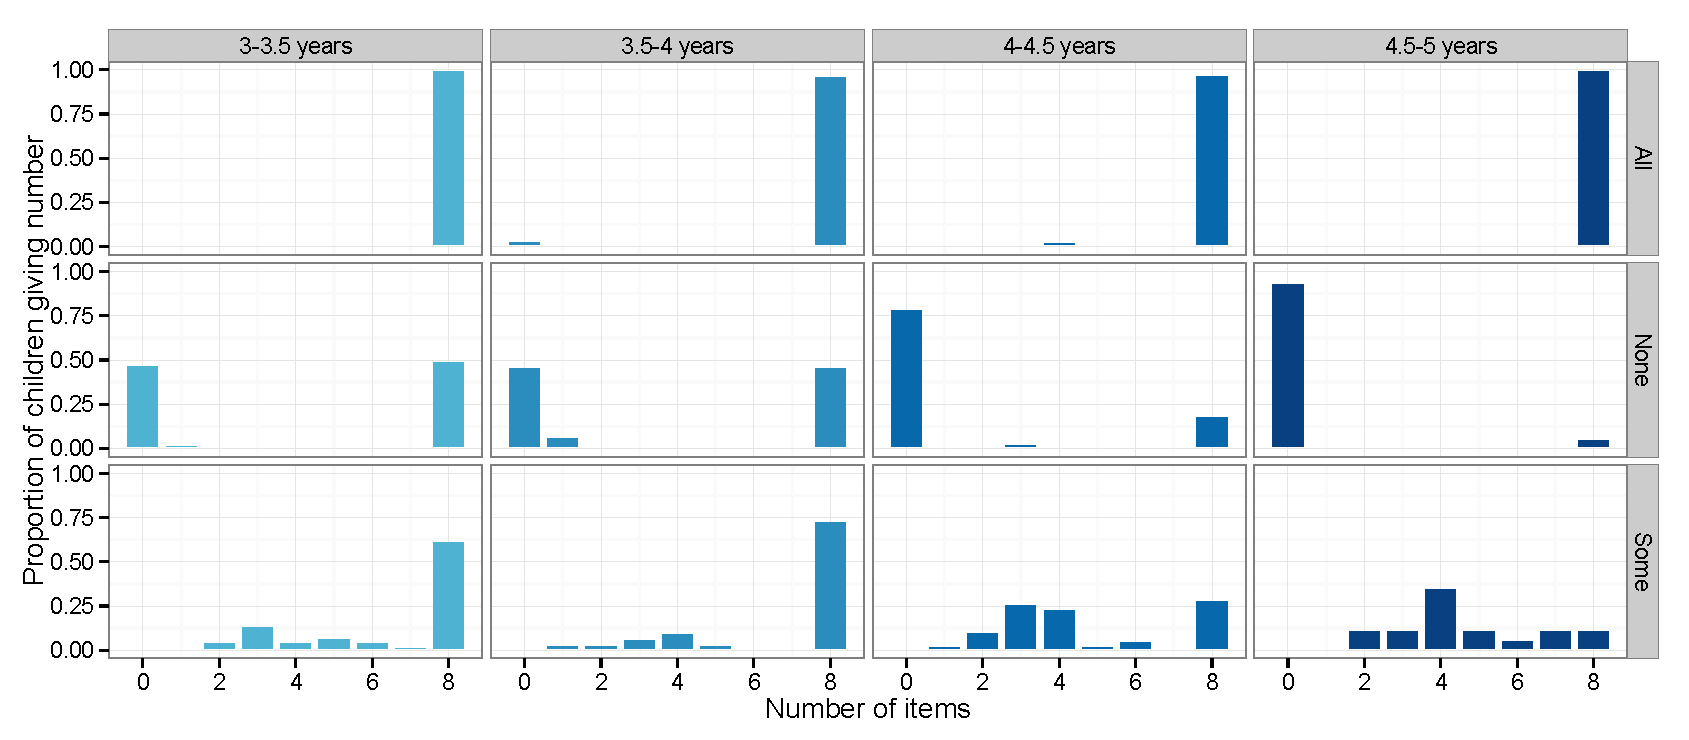
\includegraphics[width = \textwidth]{figures/exp3_GQspread.pdf} 
  \caption{\label{fig:GQ_spread} Proportion of children giving numbers of items faceted by age group and quantifier prompts \textit{all, most, none} and \textit{some}.} 
 \end{center} 
\end{figure}


\begin{figure} 
 \begin{center} 
  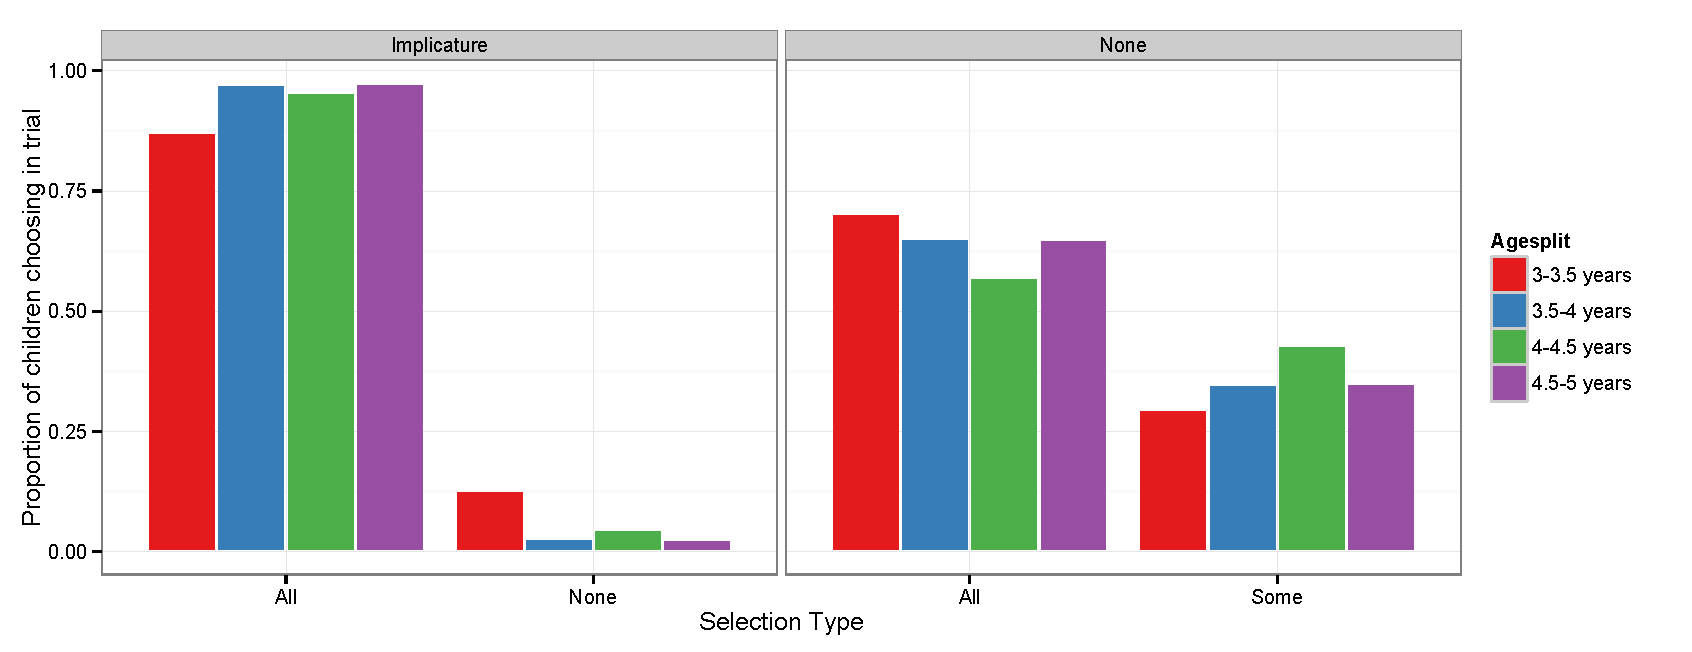
\includegraphics[height=2in]{figures/exp3_wrong.pdf} 
  \caption{\label{fig:exp3_wrong} Proportion of children choosing an alternative on incorrect trials, faceted by trial type (\textit{some, none}) and split by age group.} 
 \end{center} 
\end{figure}

In a further exploration of the relationship between quantifier knowledge and scalar implicature performance, we examined both the particular kinds of errors that children made across both tasks, and how they were related. Figure \ref{fig:exp3_wrong} shows the breakdown of children's performance in our Scalar Implicature task on incorrect trials. As in Experiment 2, children seemed to make their selections based on the target noun rather than the scalar description. This result closely mirrors children's performance in our Give-Quantifier task (Figure \ref{fig:GQ_spread}), in which younger children responded in a binomial fashion for the items \textit{some} and \textit{none}. 

In a planned logistic regression, we tried to predict performance on the implicature task from inhibitory control, quantifier knowledge, and age. When collapsing across trial types in both the implicature and quantifier tasks, we found a main effect of performance on Give-Quantifier ($\beta$ = .62, \emph{p} $<$ .05). In attempting to predict performance on trial type on the basis on quantifier knowledge, and age, we found that performance on \emph{none} trials in the implicature task was significantly predicted by Give-Quantifier \emph{none} trials ($\beta$ = 2.9, \emph{p} $<$ .001), but only marginally predictive in \emph{some} trial ($\beta$ = .99, \emph{p} = .09). 

In partial-correlations controlling for age, we found that performance on our Give-Quantifier and implicature tasks were correlated: children who tended to struggle with scalar terms in the context of implicatures also had lower performance when asked to produce a number of items in response to a quantifier prompt, specifically on \textit{some}  (\textit{r} = .27, \textit{p} $<$ .02) and \textit{none} trials in both tasks {\textit{r} = .52, \textit{p} \textless .0001). We did not find a significant correlation with performance on \textit{some} implicature and \textit{none} quantifier trials (\textit{r} = .18, \textit{p} = .14), although we did find a relation between performance on \textit{none} implicature and \textit{some} quantifier trials (\textit{r} = .35, \textit{p} = .002). 



\subsection{Discussion}

In Experiment 3, we turned our attention to investigating potential factors behind children's difficulty with making scalar implicatures. We combined two tasks targeting specific hypothesized areas of difficulty (inhibitory control and lack of quantifier knowledge) with our implicature paradigm in a within-subjects design to explore the relationship amongst these abilities. 

While we found that younger children did have difficulties in our inhibitory control task, we did not find a significant relation between performance in this task and our other tasks on the basis of inhibitory control. 

We did find that children's performance on the Give-Quantifier and Implicature tasks were related, and children who failed with scalar items tended to do so across both tasks. This result indicates that processing quantifiers is difficult for children even removed from making implicatures. While it is clear that children struggle with quantifier comprehension, the source of this developmental difficulty is less clear. It is still possible that children's definitions of these scalar terms are not solidified in the pre-school years, and that successfully understanding \textit{some} necessitates understanding both \textit{none} and \textit{all}. It is also possible that the pragmatic contexts in which these scalar items occur are particularly difficult to process, and may require excessive processing time and effort on behalf of the child. 

\section{General Discussion}

We designed a simple task to test children's sensitivity to a variety of word choice cues in a single paradigm, allowing us to investigate patterns of pragmatic development both within- and between-subjects. We minimized task demands by asking participants to select the speaker's intended referent from among three visual alternatives. In Experiment 1, we replicated the finding that preschoolers can compute ad-hoc implicatures, though we found poor performance on scalar implicatures. In Experiment 2, preschoolers' comprehension of all scalar quantifier terms in the task increased with age, and removing the ad-hoc trials increased older children's performance on scalar implicature. In Experiment 3, we explored two possible sources of difficulty in implicature computation, inhibitory control and quantifier knowledge, and found that even when removed from an implicature context, quantifier comprehension is difficult for children.  Our findings suggest that 4-year-olds are able to compute scalar implicatures with support from contextual cues, but their performance is fragile and may be inhibited by an unestablished quantifier scale.

Our work contributes to the existing literature in a number of ways. First, it offers a novel paradigm that is less complicated than many other implicature tasks, leading us to feel more confident that our results reflect children's true sensitivity rather than inadvertent task demands. Each test set remained visible to children, and they were merely asked to select which picture they thought was the referent of the speaker's description. Second, the relatively high number of trials both helped strengthen our analytical power and also offered the possibility for children to identify lexical alternatives as the study progressed (although we did not find that their performance significantly changed over the course of either experiment, cf. \citeNP{skordos2014}). Third, we were able to not only compare performance across age groups, but also examine individual patterns of responses across the different trial types. This design helped us determine that preschoolers' performance on scalar implicature trials was bimodal and highly related to their performance on \emph{none} trials, which we would have been unlikely to uncover in a purely between-subjects implicature design without controls. Finally, we were able to explicitly test two hypotheses about the sources of children's difficult with scalar implicatures, and rule out pure inhibition as a reason for failure.

Our findings also support the Alternatives Hypothesis \cite{barner2010,barner2011}. First, our ad-hoc trials in Experiment 1 show that preschoolers had no difficulty generally making inferences about contextual descriptions when alternative descriptions are obvious from the context. Performance on scalar trials also appeared to be related to the recognition of a broad set of lexical alternatives, due to both preschoolers' increasing ability to compute scalar implicatures with age (presumably a proxy for familiarity with scalemates) and due to the difference in performance across Experiments 1 and 2. Overall, these patterns of results support the idea that children's ability to compute implicatures relates to their ability to reason about what other possible utterances a speaker could have used instead. One pattern in our data is more difficult to reconcile with the Alternatives Hypothesis: Children's performance did not change over the course of either experiment. We had expected that, if children's difficulties with scalar implicature were due to a lack of recognition of the contrastive relationship between ``some'' and ``all,'' that this relationship would be revealed by the two words' consistent use in contrasting references over the course of the many trials that each child completed  \cite{skordos2014}. 

The correlated responses for \emph{none} and \emph{some} trials in both Experiments 1 and 2 presented an interesting puzzle which we addressed in Experiment 3. \emph{None} is not typically considered part of the same Horn scale as \emph{some} and \emph{all} (because ``all'' entails \emph{some}, but ``some'' does not entail \emph{none}---and in fact entails the opposite), but it is nonetheless a lexical contrast along the same quantifier scale. One possibility is that children's knowledge of the whole quantifier scale plays a role in scalar implicature, though knowledge of logically-false alternatives is not involved in the computations outlined by most theoretical accounts of \cite<e.g.>{barner2011}. Another is that performance on \emph{none} and \emph{some} trials may be correlated because both scalar implicature and negation comprehension might require inhibiting another response---the positive alternative in the negative case, and the stronger alternative in the implicature case. In our exploration of these two alternatives, we found support for the possibility that quantifier knowledge, rather than inhibitory control, drives the pattern of performance that we observed in our studies. 

Several limitations in the current study provide direction for further work. First, in coding children's performance on DCCS, we did not record children's response time. It is possible that a more nuanced measure of inhibitory control (response latencies) might yield more information about the particular processing and inhibitory demands that these implicatures entail. Additionally, our quantifier knowledge measure \cite{barner2009} may present many of the same pragmatic hurdles as our implicature task.  Future work will pursue response latencies as an alternative measure of inhibitory control in addition to exploring to what extent children's difficulty with \emph{some} and \emph{none} are the result of challenging pragmatic contexts. While our results indicate that children's failure in scalar implicature tasks may have a root in absent quantifier knowledge, it is still very likely that the sources of developmental difficulty with implicatures come from several areas.

% 'the cognitive control to select the appropriate implied referent. 
%INHIBITORY CONTROL? 

%though suggests that there may be more to the picture of children's ability to compute scalar implicatures. Our ad-hoc trials in Experiment 1 indicate that preschoolers had no difficulty making inferences about contextual descriptions, giving support that they evaluated the speaker's intended meaning when able to consider the possible descriptive choices for the visual alternatives; children tailored their selections to the speaker's most likely referent based on her choices of words given the potential items to be named in the scene. 

%For the scalar trials, we also see evidence that performance was based on recognition of lexical alternatives: preschoolers' ability to compute scalar implicatures increases with age (presumably a proxy for familiarity with these scalemates). Additionally, the correlated bimodal pattern of responses for \emph{some} and \emph{none} trials in both Experiments 1 and 2 indicates that children's inferences are related to their comprehension of related lexical alternatives. \emph{None} is not typically considered part of the same Horn scale as \emph{some} and \emph{all} (because ``all'' entails \emph{some}, but ``some'' does not entail \emph{none}---and in fact entails the opposite), but it is nonetheless a lexical contrast along the same quantifier scale. Overall, these patterns of results support the idea that children's ability to compute implicatures relates to their ability to consider what other possible utterance choices a speaker could have used instead.  As children gain more experience with language and members of the same quantifier scale, they are more likely to succeed in making inferences about the implications of these particular word choices. 


 % were sensitive to opportunities for inferences based on contrasts in lexical choices, that their level of implicature performance should increase over the course of the experiment. In other words, because children comprehend ``all,'' they should infer that the speaker's choice to use ``all'' in some trials but ``some'' and ``none'' in others implies that she intends a reference other than \emph{all} by these alternative descriptions. This logic could be a lower-level lexical inference (that ``all'' and ``some'' or ``none'' should not overlap in meaning), or a pragmatic inference (that if the speaker has selectively used ``all'' on certain trials and uses ``some'' or ``none'' on other trials, she probably intended a different meaning by using these different terms). Either route to inference should make children more likely to select the picture that is \emph{not} ``all'' on \emph{some} and \emph{none} trials, leading to an increase in correct target selections for ``some'' (which still pictures the named item). 
The lack of trial order effects we observed could indicate that children in our task did not yet have strong enough comprehension of these terms for contrastive use to matter, or alternatively that our referent-selection task eliminated the problem of summoning the contrasting term to mind and instead foregrounded some other inferential challenge (perhaps that of inhibitory control). 
% , do not recognize them as lexical alternatives, or do not perceive descriptive changes as indicators of contrast relevant to the context. 

% The simple pictures in our task may have also influenced children's ability to interpret the speaker's descriptions, as adults rate quantifier use for small numbers as less natural than for larger numbers \cite{degen2014b}. 


%Because we don't see a change in performance across trials, it may be the case that children need stronger lexical knowledge of particular terms before making inferences purely on contrastive word choice. It may not be enough just to hear that a speaker is using different words, and may be the case that children need more evidence about the particular meanings of these terms before they can demonstrate inferences about changes in their implied meaning. 


%In other words, even if children were not complete comprehenders of ``some'' and ``none'', they should realize that, across the first few trials, that if they know the meaning of \emph{all} (at which they perform near ceiling), then they should be able to make the inference that a change in quantifier (``some'' or ``none'' in place of ``all'') should indicate a change in meaning (that another quantifier should not \emph{also} refer to the picture of \emph{all}).  

% In sum, sensitivity to speaker's word choices can facilitate the information exchange between conversational patterers. 
% Implicatures are particularly useful instances of pragmatic inferences because they involve \emph{implied} meaning, offering opportunities for a inference with high likelihoods of success when recognized compared with more subtle uses of language. 
In sum, our work suggests that children can draw implicatures based on some lexical choices---such as in the case of ad-hoc implicatures---but they still struggle with quantifier-based scalar implicatures until relatively late. This difficulty is not confined to making scalar implicatures, but extends to children's knowledge of the quantifiers \emph{some} and \emph{none}. The particular trouble with these two quantifiers seems to be rooted in incomplete quantifier knowledge rather than inhibitory control. Once children understand the full quantifier scale, they can recognize the relevant category contrasts intended and compute implicatures from these quantifier word choices. 
% than the pragmatic cues of varying descriptive choices. Children may need to have a stronger comprehension of a lexical category before making inferences about possible within-category distinctions word choices convey.  Once they can recognize the relevant category contrasts intended, they can compute implicatures from these word choices. 




\bibliographystyle{apacite2}
\bibliography{biblibrary}

\newpage
\theappendix 

\section{}

\end{document}